\documentclass[12pt]{article}

\title{Activity 7: Hello, Python!}
\author{Dr. Chris Mayfield}
\date{CS 101, Fall 2017}

%\ProvidesPackage{cspogil}

% fonts
\usepackage[utf8]{inputenc}
\usepackage[T1]{fontenc}
\usepackage{mathpazo}

% spacing
\usepackage[margin=2cm]{geometry}
\renewcommand{\arraystretch}{1.4}
\setlength{\parindent}{0pt}

% orphans and widows
\clubpenalty=10000
\widowpenalty=10000
\pagestyle{empty}

% figures and tables
\usepackage{graphicx}
\usepackage{multicol}
\usepackage{tabularx}
\usepackage{wrapfig}

% fixed-width columns
\usepackage{array}
\newcolumntype{L}[1]{>{\raggedright\let\newline\\\arraybackslash\hspace{0pt}}m{#1}}
\newcolumntype{C}[1]{>{\centering\let\newline\\\arraybackslash\hspace{0pt}}m{#1}}
\newcolumntype{R}[1]{>{\raggedleft\let\newline\\\arraybackslash\hspace{0pt}}m{#1}}

% include paths
\makeatletter
\def\input@path{{Models/}{../../Models/}}
\graphicspath{{Models/}{../../Models/}}
\makeatother

% colors
\usepackage[svgnames,table]{xcolor}
\definecolor{bgcolor}{HTML}{FAFAFA}
\definecolor{comment}{HTML}{007C00}
\definecolor{keyword}{HTML}{0000FF}
\definecolor{strings}{HTML}{B20000}

% table headers
\newcommand{\tr}{\bf\cellcolor{Yellow!10}}

% syntax highlighting
\usepackage{textcomp}
\usepackage{listings}
\lstset{
    basicstyle=\ttfamily\color{black},
    backgroundcolor=\color{bgcolor},
    numberstyle=\scriptsize\color{comment},
    commentstyle=\color{comment},
    keywordstyle=\color{keyword},
    stringstyle=\color{strings},
    columns=fullflexible,
    keepspaces=true,
    showlines=true,
    showstringspaces=false,
    upquote=true
}

% code environments
\newcommand{\java}[1]{\lstinline[language=java]{#1}}%[
\lstnewenvironment{javalst}{\lstset{language=java,backgroundcolor=}}{}
\lstnewenvironment{javabox}{\lstset{language=java,frame=single,numbers=left}\quote}{\endquote}

% PDF properties
\usepackage[pdftex]{hyperref}
\urlstyle{same}
\makeatletter
\hypersetup{
  pdftitle={\@title},
  pdfauthor={\@author},
  pdfsubject={\@date},
  pdfkeywords={},
  bookmarksopen=false,
  colorlinks=true,
  citecolor=black,
  filecolor=black,
  linkcolor=black,
  urlcolor=blue
}
\makeatother

% titles
\makeatletter
\renewcommand{\maketitle}{\begin{center}\LARGE\@title\end{center}}
\makeatother

% boxes [optional height]
\newcommand{\emptybox}[1][10em]{
\vspace{1em}
\begin{tabularx}{\linewidth}{|X|}
\hline\\[#1]\hline
\end{tabularx}}

% models
\newcommand{\model}[1]{\section{#1}\nopagebreak}
\renewcommand{\thesection}{Model~\arabic{section}}

% questions
\newcommand{\quest}[1]{\subsection*{Questions~ (#1)}}
\newcounter{question}
\newcommand{\Q}{\vspace{1em}\refstepcounter{question}\arabic{question}.~ }
\renewcommand{\thequestion}{\#\arabic{question}}

% sub-question lists
\usepackage{enumitem}
\setenumerate[1]{label=\alph*)}
\setlist{itemsep=1em,after=\vspace{1ex}}

% inline answers
\definecolor{answers}{HTML}{C0C0C0}
\newcommand{\ans}[1]{%
\ifdefined\Student
    \leavevmode\phantom{~~\textcolor{answers}{#1}}
\else
    ~~\textcolor{answers}{#1}
\fi}

% longer answers [optional height]
\newsavebox{\ansbox}
\newenvironment{answer}[1][4em]{
\nopagebreak
\begin{lrbox}{\ansbox}
\begin{minipage}[t][#1]{\linewidth}
\color{answers}
}{
\end{minipage}
\end{lrbox}
\ifdefined\Student
    \phantom{\usebox{\ansbox}}%
\else
    \usebox{\ansbox}%
\fi}


\begin{document}

\maketitle

``By the way, the language is named after the BBC show `Monty Python's Flying Circus' and has nothing to do with reptiles.
Making references to Monty Python skits in documentation is not only allowed, it is encouraged!''
(Source:~\url{https://docs.python.org/2/tutorial/appetite.html})

\model{Using IDLE}

``IDLE is Python's Integrated Development and Learning Environment.
It has two main window types: the Shell window and the Editor window.
It is possible to have multiple editor windows simultaneously.''
(Source:~\url{https://docs.python.org/2/library/idle.html})

\bigskip
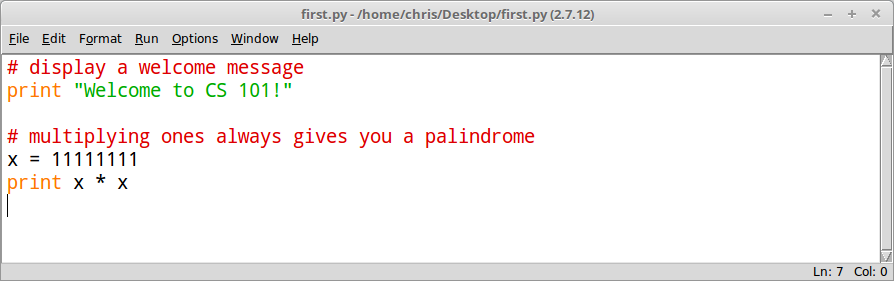
\includegraphics[width=0.8\linewidth]{idle-editor.png}

\bigskip
\hfill 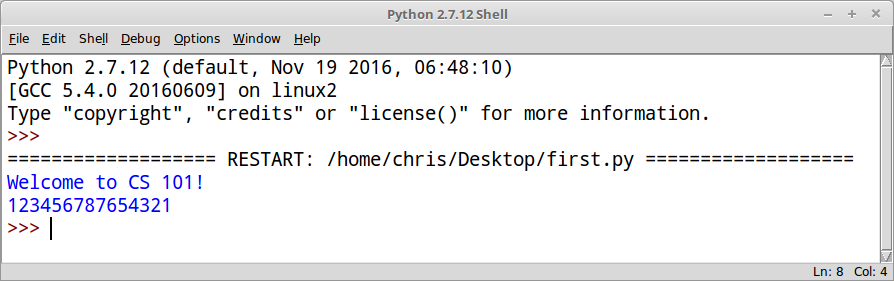
\includegraphics[width=0.8\linewidth]{idle-shell.png}


\quest{15 min}


\Q Which of the two screenshots in \ref{idle.tex} is the Shell window?
Which is the Editor window?

\begin{answer}
The top window is the editor, and the bottom window is the shell.
You can tell based on the window titles.
\end{answer}


\Q Explain the terms ``Editor'' and ``Shell'' based on what you learned previously in the course.

\begin{answer}
An editor is a simple program for writing plain text files.
A shell (or terminal) is an interface for running commands.
\end{answer}


\Q What is the name of the file in the editor? What directory is it saved in?

\begin{answer}
The name is first.py, and the directory is Desktop.
\end{answer}


\Q Explain the Python code in the editor window. What does each line do?

\begin{answer}[5em]
The first line is a comment, the second line displays a message, the third line is blank, the fourth line is another comment, the fifth line creates a variable named x, and the sixth line displays the value of x squared.
\end{answer}


\Q What is the output of the program? Where should you look for output?

\begin{answer}[5em]
The output is in the shell window (in blue): \\[2pt]
\hspace*{2em} Welcome to CS 101! \\
\hspace*{2em} 123456787654321
\end{answer}


\Q Predict the output of each line below. Then type each line into the Shell window (one at a time) and check your answers.

\begin{enumerate}
\item \pyth{print 2 * 5} \ans{10}
\item \label{add} \pyth{print 2 + 5} \ans{7}
\item \label{str} \pyth{print "2 + 5"} \ans{2 + 5 ~ (without quotes)}
\item \label{err} \pyth{print CS rocks!} \ans{SyntaxError: invalid syntax}
\item \pyth{print 2 # 5} \ans{2 ~ (because \pyth{#} makes a comment)}
\end{enumerate}

\Q Explain the difference between \ref{add} and \ref{str} in the last question. Why are the results different?

\begin{answer}
\pyth{2 + 5} computes the number 7, whereas \str{2 + 5} is literal text.
\end{answer}


\Q What is wrong with the code in \ref{err}? Explain the error message. How do you fix the error?

\begin{answer}
It's interpreting the code \pyth{CS rocks!} as an arithmetic expression, but it's not valid (e.g, there's no operator). Syntax error means the code is not correctly structured. Add quote marks around \str{CS rocks!} to fix that line.
\end{answer}

\model{Guessing Game}

Create a new file named \texttt{guess.py} and enter the following code.
Replace the name in Line~2 with your own name.
Be careful to type the code \emph{exactly} as shown.

\begin{pythbox}
name = raw_input("What is your name? ")
if name == "Taylor":
    print name, "is a great name!"
else:
    print name, "is an okay name."
\end{pythbox}

Note: \verb|raw_input| is a \textbf{function} that displays a \textbf{prompt} on the screen and reads a line from the keyboard.
In this program, the result of \verb|raw_input| is stored in the \textbf{variable} \pyth{name}.


\quest{15 min}


\Q What is the prompt? Why is there a space at the end of it?

\begin{answer}[3em]
The prompt is \str{What is your name? }.
The space at the end makes it so that the input isn't ``touching'' the question mark when the user types.
\end{answer}


\Q Run the program a few times, entering a different name each time. Feel free to modify the messages as you see fit.

\vspace{1em}


\Q Enter each of these lines into the IDLE shell, and explain where the syntax error occurs.

\begin{enumerate}[itemsep=1ex]
\item \verb|name? = raw_input("What is your name?")|
\ans{question mark}

\item \verb|your name = raw_input("What is your name?")|
\ans{space between your and name}

\item \verb|1st_name = raw_input("What is your name?")|
\ans{the word 1st}

\item \verb|from = raw_input("Where were you born?")|
\ans{equals sign (from is a keyword)}
\end{enumerate}


\Q Based on the errors in the previous question and the following correct examples, describe three rules that need to be followed when naming a variable.

\begin{pythlst}
    name2 = raw_input("What is your name?")
    your_name = raw_input("What is your name?")
    firstName = raw_input("What is your name?")
\end{pythlst}

\begin{answer}
Answers may include: it can't have punctuation or other symbols, it has to be one word, it can't start with a number, and it can't be a keyword.
\end{answer}


\Q \label{vars} At the end of your \texttt{guess.py} program, create two new variables named \pyth{number} and \pyth{guess}.
Set the value of \pyth{number} to be an integer between 1 and 100 (of your choice).
Ask the user to guess your number, and store the result in \pyth{guess}.
When asking for numbers, use \pyth{input} instead of \pyth{raw_input}.
Write your two statements in the space below.

\begin{answer}[3em]
\begin{pythans}
number = 74  # or some other value
guess = input("Guess my number: ")
\end{pythans}
\end{answer}


\Q Add the following logic to your program:
If the guess is too high, display the message \str{Too high!};
if the guess is too low, display the message \str{Too low!};
if the user guessed the number, display \str{You got it!}.
Write your statements in the space below.

\begin{answer}[8em]
\begin{pythans}
    if guess < number:
        print "Too low!"
    if guess > number:
        print "Too high!"
    if guess == number:
        print "You got it!"
\end{pythans}
\end{answer}


\Q What is the difference between \pyth{=} and \pyth{==} in the programs you have written today?

\begin{answer}[3em]
The \pyth{=} operator is used to \emph{assign} values to variables, whereas the \pyth{==} operator is used to \emph{compare} values for equality.
\end{answer}


\Q At this point, you should have a program that allows the user to make only one guess.
Rather than run this program over and over again, you can use a \pyth{while} loop to make it repeat the guessing part.
Insert the following two lines before the \pyth{input} line you wrote in \ref{vars}.

\begin{pythlst}
    guess = -1
    while guess != number:
\end{pythlst}

\vspace{1em}


\Q What did you have to do after inserting the \pyth{while} loop to make it work?
In other words, how did you make the \pyth{input} and \pyth{if} statements part of the \pyth{while} loop?

\begin{answer}
You need to indent the corresponding lines of code underneath it.
Select the rest of the program lines, and then press the Tab key.
\end{answer}


\Q Rather than guess the same number every time, you can have the computer select a random number for you:
\begin{itemize}[itemsep=2pt]
\item At the top of your program, add the line ``\pyth{import random}'' (without the quotes).
\item Then change the line where you set value of \pyth{number} to use this example instead:
\begin{pythlst}
number = random.randint(1, 100)
\end{pythlst}
\end{itemize}


\end{document}
